\section{A Small Worked Example}
\label{sec:example}

This section details a fully worked seven-vertex example to concretely illustrate our theoretical framework. While small in scale, this example exhibits all the core features of the general theory: both cone and base generators are present, the labeled violation kernel $\ker V$ is nontrivial, a presentation redundancy in the generator combinations is factored out by mapping the kernel through the mask projection to obtain the feasible branch shift space $\mathcal{K}_F = M(\ker V)$, and one free branch decision contributes a nontrivial factor $2^f$ to the final count.

\subsection{Combinatorial Setup}
\label{sec:example-combo}

Let $K=2$ in $\mathbb{R}^2$. For readability in this example, write $v_i$ for the vertex with global label $i$. The fixed initial clique is $V_0=\{v_1, v_2\}$. Consider the predecessor sets
\[
U_3=\{v_1, v_2\},
\qquad
U_4=\{v_1, v_3\},
\qquad
U_5=\{v_1, v_3\},
\qquad
U_6=\{v_1, v_4\},
\qquad
U_7=\{v_1, v_2\},
\]
and the pruning edge set
\[
E_P=\{\{v_3, v_6\},\,\{v_4, v_5\}\}.
\]
The pruning-relevant vertex set is
\[
L=\{v_1,v_2,v_3,v_4,v_5,v_6\}.
\]
The added vertex $v_7$ is not in the fixing set of any pruning endpoint, so the constrained and free branch sets are
\[
B_{\mathrm{c}}=\{v_3, v_4, v_5, v_6\},
\qquad
B_{\mathrm{f}}=\{v_7\},
\qquad
f=1.
\]
There are three predecessor cliques,
\[
C_0=\{v_1, v_2\},
\qquad
C_1=\{v_1, v_3\},
\qquad
C_2=\{v_1, v_4\}.
\]
The first is the predecessor clique for $v_3$ and the free vertex $v_7$, but only $v_3$ contributes to the constrained generator masks. The second generates $v_4$ and $v_5$, and the third generates $v_6$. Since $v_4$ and $v_5$ depend on $v_3$, and $v_6$ depends on $v_4$, we have
\[
\operatorname{Cone}(v_3)\cap B_{\mathrm{c}}=\{v_3,v_4,v_5,v_6\},
\qquad
\operatorname{Cone}(v_4)\cap B_{\mathrm{c}}=\{v_4, v_6\}.
\]
The free vertex has $\operatorname{Cone}(v_7)\cap B_{\mathrm{c}}=\varnothing$, so its branch decision does not appear in the constrained matrices below.
The graph structure, predecessor dependency arcs, and pruning edges are illustrated in Figure~\ref{fig:worked-example}.

\begin{figure}[htbp]
\centering
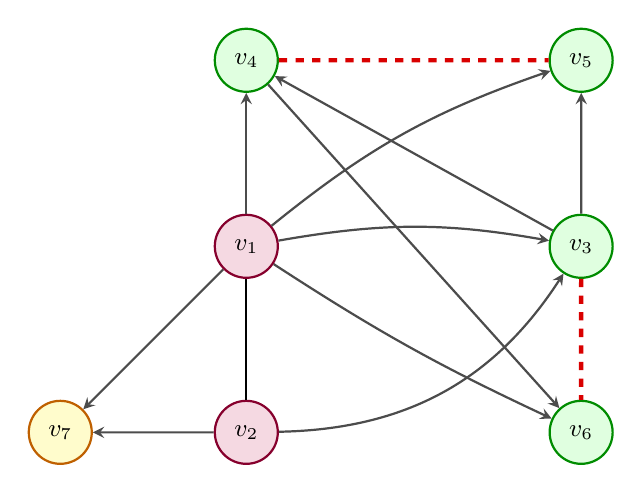
\begin{tikzpicture}[
    scale=1.05,
    >=stealth,
    every node/.style={circle, draw, minimum size=8mm, inner sep=0pt, font=\small},
    seed/.style={fill=purple!15, draw=purple!70!black, line width=0.8pt},
    constrained/.style={fill=green!12, draw=green!55!black, line width=0.8pt},
    free/.style={fill=yellow!20, draw=orange!75!black, line width=0.8pt},
    dep/.style={->, thick, black!70},
    prune/.style={dashed, ultra thick, red!85!black}
]
    % Nodes
    \node[seed] (v1) at (0,0) {$v_1$};
    \node[seed] (v2) at (0,-2.25) {$v_2$};
    \node[constrained] (v3) at (4.05,0) {$v_3$};
    \node[constrained] (v4) at (0,2.25) {$v_4$};
    \node[constrained] (v5) at (4.05,2.25) {$v_5$};
    \node[constrained] (v6) at (4.05,-2.25) {$v_6$};
    \node[free] (v7) at (-2.25,-2.25) {$v_7$};
    
    % Initial clique edge
    \draw[thick] (v1) -- (v2);
    
    % Predecessor arcs (directed)
    \draw[dep] (v1) to[bend left=10] (v3);
    \draw[dep] (v2) to[bend right=28] (v3);

    \draw[dep] (v1) to (v4);
    \draw[dep] (v3) to (v4);
    
    \draw[dep] (v1) to[bend left=10] (v5);
    \draw[dep] (v3) to (v5);
    
    \draw[dep] (v1) to[bend right=4] (v6);
    \draw[dep] (v4) to (v6);

    \draw[dep] (v1) to (v7);
    \draw[dep] (v2) to (v7);
    
    % Pruning edges (dashed red)
    \draw[prune] (v4) to (v5);
    \draw[prune] (v3) to (v6);
\end{tikzpicture}
\caption{Combinatorial predecessor dependency graph and pruning edges for the 7-vertex worked example; node positions are schematic. Directed arcs represent predecessor discretization constraints ($E_D$), dashed red lines represent $E_P = \{\{v_3, v_6\}, \{v_4, v_5\}\}$, purple nodes form $V_0$, green nodes are branch-decision vertices in $B_{\mathrm{c}}$, and the yellow node is the free branch vertex $v_7\in B_{\mathrm{f}}$.}
\label{fig:worked-example}
\end{figure}

The generator supports and associated mirror cliques are listed in Table~\ref{tab:generators}. The constrained rows are ordered as $(v_3,v_4,v_5,v_6)$, and the columns are ordered as $(g_3,g_4,g_5,g_6,g_{C_0},g_{C_1},g_{C_2})$. The free branch bit $v_7$ is intentionally omitted from these constrained masks.

\begin{table}[htbp]
\centering
\caption{Generator supports and mirror cliques for the worked example. Each support mask $S_g$ is a subset of $B_{\mathrm{c}} = \{v_3, v_4, v_5, v_6\}$; the rows define the columns $(g_3,g_4,g_5,g_6,g_{C_0},g_{C_1},g_{C_2})$ of the mask matrix $M$.}
\label{tab:generators}
\begin{tabular}{lcc}
\toprule
Generator & Support Mask ($S_g$) & Mirror Clique ($C_g$) \\
\midrule
$g_3$ & $\{v_3, v_4, v_5, v_6\}$ & $C_0 = \{v_1, v_2\}$ \\
$g_4$ & $\{v_4, v_6\}$ & $C_1 = \{v_1, v_3\}$ \\
$g_5$ & $\{v_5\}$ & $C_1 = \{v_1, v_3\}$ \\
$g_6$ & $\{v_6\}$ & $C_2 = \{v_1, v_4\}$ \\
$g_{C_0}$ & $\{v_3, v_4, v_5, v_6\}$ & $C_0 = \{v_1, v_2\}$ \\
$g_{C_1}$ & $\{v_4, v_5, v_6\}$ & $C_1 = \{v_1, v_3\}$ \\
$g_{C_2}$ & $\{v_6\}$ & $C_2 = \{v_1, v_4\}$ \\
\bottomrule
\end{tabular}
\end{table}

The generator mask matrix is
\[
M=
\begin{bmatrix}
1&0&0&0&1&0&0\\
1&1&0&0&1&1&0\\
1&0&1&0&1&1&0\\
1&1&0&1&1&1&1
\end{bmatrix}.
\]

The active edge set for the constrained subproblem is $F = E_D[L] \cup E_P$. Besides the fixed seed clique edge $\{v_1,v_2\}$, the discretization edges induced on $L$ are
\[
\{v_1, v_3\},\{v_2, v_3\},
\{v_1, v_4\},\{v_3, v_4\},
\{v_1, v_5\},\{v_3, v_5\},
\{v_1, v_6\},\{v_4, v_6\}.
\]
The nonzero labeled active-edge violations are summarized in Table~\ref{tab:violations}.

\begin{table}[htbp]
\centering
\caption{Labeled active-edge violations for each generator. The entry \textnormal{none} means that the generator contributes no row to the labeled violation matrix $V$; the nonzero rows are indexed by $(\{v_4,v_5\},C_1)$ and $(\{v_3,v_6\},C_2)$.}
\label{tab:violations}
\begin{tabular}{lcc}
\toprule
Generator & Violated Active Edge ($e$) & Mirror Label ($C_g$) \\
\midrule
$g_3$ & \text{none} & \text{none} \\
$g_4$ & $\{v_4, v_5\}$ & $C_1$ \\
$g_5$ & $\{v_4, v_5\}$ & $C_1$ \\
$g_6$ & $\{v_3, v_6\}$ & $C_2$ \\
$g_{C_0}$ & \text{none} & \text{none} \\
$g_{C_1}$ & \text{none} & \text{none} \\
$g_{C_2}$ & $\{v_3, v_6\}$ & $C_2$ \\
\bottomrule
\end{tabular}
\end{table}

Thus, with rows ordered as the two active-edge labels $(\{v_4, v_5\},C_1)$ and $(\{v_3, v_6\},C_2)$, the labeled violation matrix is
\[
V=
\begin{bmatrix}
0&1&1&0&0&0&0\\
0&0&0&1&0&0&1
\end{bmatrix}.
\]
Write a generator coefficient vector as $\alpha = (a_3,a_4,a_5,a_6,a_{C_0},a_{C_1},a_{C_2}) \in \mathbb{F}_2^7$. Then the zero-violation condition $V\alpha = 0$, with arithmetic over $\mathbb{F}_2$, is equivalent to
\[
a_4+a_5=0,
\qquad
a_6+a_{C_2}=0.
\]
Hence, $a_4=a_5=t$, $a_6=a_{C_2}=u$, and $a_3,a_{C_0},a_{C_1}$ are free. Applying the mask matrix gives
\[
M\alpha
=
t(m_4+m_5)+u(m_6+m_{C_2})+a_3m_3+a_{C_0}m_{C_0}+a_{C_1}m_{C_1}.
\]
The parameter $u$ changes the generator presentation but not the branch mask, because $m_6=m_{C_2}$. Also $m_3=m_{C_0}$ and $m_4+m_5=m_{C_1}$. Therefore,
\[
\mathcal{K}_F
=
M(\ker V)
=
\left\{
\begin{bmatrix}0\\0\\0\\0\end{bmatrix},
\begin{bmatrix}1\\1\\1\\1\end{bmatrix},
\begin{bmatrix}0\\1\\1\\1\end{bmatrix},
\begin{bmatrix}1\\0\\0\\0\end{bmatrix}
\right\}.
\]
The ranks are
\[
\operatorname{rank}_{\mathbb{F}_2}\begin{bmatrix} M \\ V \end{bmatrix}=4,
\qquad
\operatorname{rank}_{\mathbb{F}_2}(V)=2.
\]
Since $f=1$, the solution count is
\[
\lvert \Xi \rvert = 2^{1+4-2} = 8.
\]
The two independent feasible constrained branch shifts are the mask $\{v_3,v_4,v_5,v_6\}$, obtained from $g_3$ or $g_{C_0}$, and the mask $\{v_4, v_5, v_6\}$, obtained from $g_4\oplus g_5$, or equivalently from the base generator $g_{C_1}$. These generate four feasible constrained codes from a reference solution. The independent free bit at $v_7$ doubles this count, giving eight full feasible branch codes.

\subsection{Concrete Geometric Realization}
\label{sec:example-geometry}

To ground this algebraic structure, we provide a concrete geometric realization in $\mathbb{R}^2$ with exact coordinates. This numerical setup illustrates how the combinatorial conditions established by our theory manifest physically as distance-preserving operations.

\paragraph{Reference Coordinate Embedding.}
We place the initial clique $V_0 = \{v_1, v_2\}$ and the branch decision vertex $v_3$ at
\[
v_1 = (0,0), \quad v_2 = (-2,0), \quad v_3 = (0,2).
\]
The remaining vertices are placed at their reference coordinates:
\[
v_4 = (1, 1), \quad v_5 = (2, 2), \quad v_6 = (2, 0), \quad v_7 = (-1,1).
\]
These coordinates determine the physical edge weights. All discretization distances are positive and can be verified directly: $d_{13} = 2$, $d_{23} = 2\sqrt{2}$, $d_{14} = d_{34} = d_{17} = d_{27} = \sqrt{2}$, $d_{15} = 2\sqrt{2}$, $d_{35} = 2$, $d_{16} = 2$, and $d_{46} = \sqrt{2}$. The two active pruning distances to be tested by our constraint matrices are
\[
d_{36} = \|v_3 - v_6\|_2 = 2\sqrt{2},
\qquad
d_{45} = \|v_4 - v_5\|_2 = \sqrt{2}.
\]
The free vertex $v_7$ contributes only its discretization distances $d_{17}$ and $d_{27}$, which do not appear in the active pruning set $F$ since $v_7 \notin L$.

\paragraph{Physical Reflection and Violation Mechanics.}
We can now trace how individual generator moves deform the embedding and interact with the pruning constraints. First, consider the cone generator $g_3$. The mirror for $v_3$ is the $x$-axis, $\operatorname{aff}(v_1, v_2)$. Activating $g_3$ reflects the downstream cone $\{v_3, v_4, v_5, v_6\}$ across this line. Because all affected vertices are reflected together and the fixed endpoints $v_1,v_2$ lie exactly on the mirror, all discretization and pruning distances are trivially preserved. Similarly, the mirror for $v_7$ is also the $x$-axis. Reflecting $v_7$ to $v_7' = (-1,-1)$ preserves its discretization distances $d_{17}$ and $d_{27}$ and has no contact with the pruning edges. This shows geometrically why the branch decision $v_7$ is completely free, contributing the independent factor $2^f = 2$ to the final solution count.

In contrast, isolated branch shifts that do not belong to the kernel $\ker V$ physically violate the pruning constraints. For instance, the mirror for $v_5$ is the $y$-axis, $\operatorname{aff}(v_1, v_3)$. Mirroring only $v_5$ across the $y$-axis yields $v_5' = (-2, 2)$. While this preserves all discretization distances, it stretches the pruning edge $\{v_4, v_5\}$ to $\|v_4 - v_5'\|_2 = \sqrt{10} \ne \sqrt{2}$, confirming a physical violation. This matches the algebraic violation matrix where $g_5$ has a $1$ in row $(\{v_4,v_5\}, C_1)$. Similarly, the cone generator $g_4$ reflects $v_4$ and its descendant $v_6$ across the $y$-axis, yielding $v_4' = (-1,1)$ and $v_6' = (-2,0)$. This preserves the discretization distance $\{v_4, v_6\}$ and the pruning distance $\{v_3, v_6\}$ (since $v_3$ lies on the $y$-axis mirror), but violates the active edge $\{v_4, v_5\}$ to length $\sqrt{10}$. Lastly, the mirror for $v_6$ is the line $y=x$, $\operatorname{aff}(v_1, v_4)$. Reflecting only $v_6$ gives $v_6' = (0,2)$, which collapses the pruning distance to $v_3$ from $2\sqrt{2}$ to $0$, mapping to the algebraic violation of $g_6$ against $\{v_3,v_6\}$.

\paragraph{Kernel-Induced Cancellation and Dynamic Mirrors.}
The core power of our framework is demonstrated when we apply the nontrivial feasible branch shift $h = \{v_4, v_5, v_6\} \in \mathcal{K}_F$, represented algebraically by the generator combination $g_4 \oplus g_5$ (or equivalently by $g_{C_1}$), where adding the redundant generator pair $g_{C_2} \oplus g_6$ yields the same branch mask. Geometrically, this shift instructs us to reflect $v_4, v_5$, and $v_6$ simultaneously across the $y$-axis ($x=0$), yielding:
\[
v_4' = (-1, 1), \quad v_5' = (-2, 2), \quad v_6' = (-2, 0).
\]
Because all three vertices are reflected by the same isometric reflection $R_{C_1}$ across the $y$-axis, the internal active distance $\|v_4' - v_5'\|_2 = \sqrt{2} = d_{45}$ is preserved. 

The interaction with the dynamic mirror of $v_6'$ reveals the beauty of this cancellation. In the original embedding, $v_6$ is placed using the mirror $\operatorname{aff}(v_1, v_4)$. Under the branch shift, $v_4$ moves to $v_4'$, so the dynamic mirror for the subsequent step rotates to $\operatorname{aff}(v_1, v_4')$, which is the line $y = -x$. The coordinates $v_6' = (-2,0)$ are the exact reflection of the reference $v_6 = (2,0)$ across the $y$-axis. Because $v_6'$ is placed symmetrically with respect to the rotated mirror $y = -x$, the discretization distances are preserved. Crucially, the pruning distance to the fixed vertex $v_3 = (0,2)$ is preserved:
\[
\|v_3 - v_6'\|_2 = \|(0,2) - (-2,0)\|_2 = 2\sqrt{2} = d_{36}.
\]
This coordinate realization illustrates how the algebraic kernel $\ker V$ maps perfectly to viable physical realizations in this system, factoring out the representation redundancies and matching the rank-count prediction.

